
Bipartite fidelity is the overlap of the groundstates of two Hamiltonians. In the path integral language, the groundstates can be produced by imaginary time evolution. If we take the horizontal axis as the Euclidean time, the fidelity can be diagrammatically represented as in Fig.~\ref{fig:fidel}. Treating it as a partition function, we analyze its finite size dependence on the total chain size $L$. The logarithmic fidelity should then follow the general discussion of Cardy and Peschel\cite{cardy_finite-size_1988} of the finite size dependence of free energy and give a term proportional to $\ln L$
\begin{equation}
\mathcal{F} = - \ln \langle \phi_1 |\phi_2 \rangle^2 = - 2 \ln Z  \sim  \ln L 
\end{equation}
The proportionality constant is the exponent characterizing the interface. 

\begin{figure}[h]
\centering
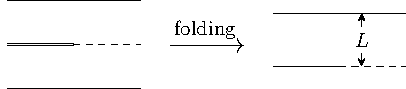
\includegraphics[width=\textwidth]{fig_fidel.pdf}
\caption{Fidelity of connecting two CFTs. The horizontal axis the imaginary time. Evolution on the two infinitely extended side produces the groundstate of the disconnected and connected chain Hamiltonians. The right diagram is the result of folding the lower part of the diagram up, so that all the boundary are now boundary states.}
\label{fig:fidel}
\end{figure}

\todo[inline]{echo diagram folding}

The Loschmidt echo is defined to be defined as the overlap of the ground state and the quenched states, 
\begin{equation}
\mathcal{L} = |\langle \phi_{\rm gnd}  | e^{-i Ht } | \phi_{\rm gnd} \rangle|^2
\end{equation}
We have drawn the path integral definition of this quantity in Fig.~\ref{fig:cut-and-join}; for convenience of the latter conformal mapping, we turn the diagram by a right angle and take the horizontal axis as time. The slits represents disconnected boundary conditions like Dirichlet and Neumann, the dashed line represent partially transmitting boundary condition parameterized by $\lambda$. We may as well fold the lower half plane up and everything on the real axis should be regarded as boundary states. Again by Cardy and Peschel\cite{cardy_finite-size_1988}, the logarithm of the Loschmidt echo is the free energy and should have logarithmic dependence on the characterizing length scale in the problem. In other words
\begin{equation}
\mathcal{L} = - \ln |\langle \phi_{\rm gnd}  | e^{-i Ht } | \phi_{\rm gnd} \rangle|^2 \propto \ln \tau 
\end{equation}



%%% Local Variables:
%%% TeX-master: "bCFT_paper"
%%% TeX-PDF-mode: t
%%% End:
